\documentclass[conference]{IEEEtran}
\usepackage[brazilian]{babel}
\usepackage[utf8]{inputenc}
\usepackage[T1]{fontenc}
\usepackage{cite}
\ifCLASSINFOpdf
\usepackage[pdftex]{graphicx}
  % declare the path(s) where your graphic files are
  % \graphicspath{{../pdf/}{../jpeg/}}
  % and their extensions so you won't have to specify these with
  % every instance of \includegraphics
  % \DeclareGraphicsExtensions{.pdf,.jpeg,.png}
\else
  % or other class option (dvipsone, dvipdf, if not using dvips). graphicx
  % will default to the driver specified in the system graphics.cfg if no
  % driver is specified.
\usepackage[dvips]{graphicx}
  % declare the path(s) where your graphic files are
  % \graphicspath{{../eps/}}
  % and their extensions so you won't have to specify these with
  % every instance of \includegraphics
  % \DeclareGraphicsExtensions{.eps}
\fi

\usepackage{adjustbox}
\usepackage{fancyvrb}

\usepackage[cmex10]{amsmath}
\usepackage{algorithmic}
\usepackage{array}
\usepackage{mdwmath}
\usepackage{mdwtab}
%\usepackage{eqparbox}
\usepackage[tight,footnotesize]{subfigure}
%\usepackage[caption=false]{caption}
\usepackage[font=footnotesize]{subfig}
%\usepackage{stfloats}
\usepackage{url}
\usepackage{csvsimple,longtable,booktabs}
\usepackage{pgfplots}
\usepackage{pgfplotstable}
\hyphenation{op-tical net-works semi-conduc-tor}
%\usepackage{listings}

%\lstset{language=C++,
%	basicstyle=\ttfamily,
%	keywordstyle=\color{blue}\ttfamily,
%	stringstyle=\color{red}\ttfamily,
%	commentstyle=\color{green}\ttfamily,
%	morecomment=[l][\color{magenta}]{\#}
%}

\begin{document}
\title{Programação de Alto Desempenho\\
\large Atividade 7 --- Programação CUDA}

\author{\IEEEauthorblockN{Lucas Santana Lellis --- 69618}
\IEEEauthorblockA{PPGCC --- Instituto de Ciência e Tecnologia\\
	Universidade Federal de São Paulo} }

% make the title area
\maketitle

%\IEEEpeerreviewmaketitle

\section{Introdução}
Nesta atividade foram realizados experimentos com programação CUDA para placas aceleradoras.
Cada experimento foi realizado 3 vezes, e os resultados apresentados são a média dos resultados obtidos em cada um deles, sendo calculado o speedup em comparação à execução em CPU.
As especificações da máquina utilizada estão disponíveis na Tabela\ref{tab:cpu}.

\begin{table}[htb!]
\centering
\begin{tabular}{ll|ll}
\bfseries CPU & Intel i7 990X & \bfseries Cores & 6\\
\bfseries Threads & 12 & \bfseries Clock & 3.47 GHz\\
\bfseries Cache& 12 MB  &\bfseries RAM & 20 GB \\
\bfseries SO & Ubuntu 14.04 & \bfseries Kernel & 3.13.0 \\
\bfseries GPU & Tesla K40 & \bfseries Threads & 2880 \\
\bfseries Mem. & 12Gb GDDR5 &\bfseries CUDA Cap. & 3.5 \\
\bfseries GCC & 4.8.5 & \bfseries NVCC & V7.5.17
\end{tabular}
\caption{Especificações da Máquina\label{tab:cpu}}
\end{table}

\section{Exercício I --- Difusão de calor\label{sec01}}
Neste exercício foi feita a paralelização em CUDA do algoritmo da difusão de calor em um domínio unidimensional através de diferenças finitas.

Foram implementados dois kernels, um para a transmissão de calor, chamado ``Atualiza'', e um para a operação de redução que retorna o valor máximo no vetor, chamado ``Maximo'', em uma versão alternativa, a inicializacao do vetor também é paralelizada pelo kernel ``Inicializacao''.

Alguns recursos do algoritmo original não foram implementados em CUDA, como o cálculo de $x$, que acumulava $dx$ à cada iteração. Além disso, a operação de redução ``Maximo'' apenas retorna o maior valor, ignorando a posição do maior valor do vetor. De qualquer forma, em ambas implementações o resultado obtido é o mesmo: $99.8486$.

No algoritmo em CUDA, foram obtidos os tempos da tabela\ref{tab:ex01-cuda}, onde \textit{HostToDevice} é o tempo de transmissão do vetor da memória local para a placa aceleradora, \textit{Tempo kernels} é o tempo total da execução da etapa de transmissão de calor, em que são feitas chamadas sucessivas do kernel ``Atualiza'', \textit{Tempo medio} é o tempo médio da execução dos kernels, \textit{DeviceToHost} é o tempo de transmissão da saída da operação de redução para a CPU, e finalmente o \textit{Tempo Total} é o tempo total da execução do algoritmo.

\begin{table}[htb!]
\centering
\begin{tabular}{rl}
\bfseries HostToDevice: & 0.000165 \\
\bfseries Tempo kernels: & 0.112622 \\
\bfseries Tempo medio: & 0.000011 \\
\bfseries DeviceToHost: & 0.012765 \\
\bfseries Tempo Total: & 0.125966 \\
\end{tabular}
\caption{Tempos obtidos na execução CUDA.\label{tab:ex01-cuda}}

\end{table}

Agora, na Tabela \ref{tab:ex01-cpu} é feita a comparação entre a execução em CPU e em GPU. O speedup da operação foi de 10 vezes se comparado à execução em apenas uma thread na CPU.


\begin{table}[htb!]
\centering
\begin{tabular}{rl}
  \bfseries CPU & 1.34425 \\
  \bfseries GPU & 0.125966 \\
  \bfseries CPU/GPU & 10.671530 \\
\end{tabular}
\caption{Comparação da execução em CUDA vs CPU.\label{tab:ex01-cpu}}
\end{table}

\section{Exercício II --- nvprof e nvvp\label{sec:ex02}}
Neste exercício utilizei o nvprof e nvvp para analisar a execução do exercício da seção\ref{sec01}. Na Figura\ref{fig:nvvp} está a saída do nvvp, e na Figura\ref{fig:nvprof} um resumo da saída do nvprof, com os argumentos ``nvprof --print-gpu-trace bin/ex01 ''.

\begin{figure*}
  \centering
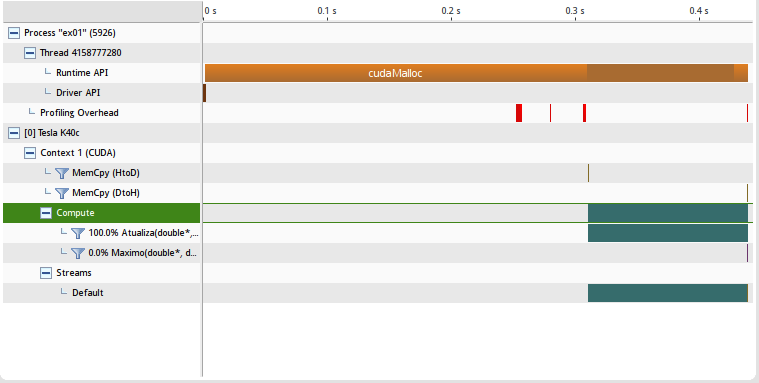
\includegraphics[width=\textwidth] {figs/nvvp}
\caption{Saída do NVVP sobre o programa em CUDA da Seção\ref{sec01}.}
\label{fig:nvvp}
\end{figure*}

Uma análise mais profunda da Figura\ref{fig:nvprof} revela algumas informações interessantes:
A transmissão dos dados iniciais para o dispositivo durou 136.39us, sendo enviados 781.25KB a uma taxa de 5.4629GB/s;
Foram realizadas 50000 chamadas do kernel ``Atualiza'', cada uma durando em torno de 9us;
A operação de redução ``Maximo'' em duas etapas, a primeira com 16us e a segunda com 4us;
Por fim, a cópia do resultado da redução que durou 3us para enviar 8 bytes à memória principal.

\section{Exercício III --- Numeros Aleatorios\label{sec:ex03}}
Nesse exercício foi implementado um kernel em CUDA para preencher um vetor com números aleatórios do tipo float utilizando a função ``cuRand''.
Neste exemplo, não foi necessário separar a etapa de atribuição das sementes da etapa de obtenção do número aleatório, uma vez que a utilização da função cuRand é realizada em apenas uma etapa em todo o código.

Foi feita uma implementação da mesma operação, utilizando a função ``rand'' para gerar um vetor de números aleatorios na CPU.
A comparação entre os tempos de execução está na Tabela\ref{tab:ex03}, e vemos que o speedup foi de 20 vezes com relação á execução em CPU com apenas uma thread.

\begin{table}[htb!]
\centering
\begin{tabular}{rl}
  \bfseries CPU & 0.010963 \\
  \bfseries GPU & 0.000534 \\
  \bfseries CPU/GPU & 20.529962\\
\end{tabular}
\caption{Comparação da execução em CUDA vs CPU.\label{tab:ex03}}
\end{table}

\section{Exercício IV --- Somatorio de Nros. Aleatorios}
Utilizando o código do exercício da Seção\ref{sec:ex03}, o exercício atual compreende no somatório dos valores de um vetor preenchido com números aleatórios. Trata-se também de uma operação de redução em CUDA, realizada de forma semelhante à Seção \ref{sec:ex02}.

Um teste simples para somar um vetor de 1000000 posições com apenas o valor 1 foi suficiente para revelar uma deficiência nessa abordagem de redução utilizada, pois o valor obtido era muito inferior ao esperado.
Logo, chegamos à conclusão que a utilização dessa função de redução para vetores com muitos elementos e blocos de tamanho fixo poderia causar resultados inconsistentes, e que para que a função de redução funcione corretamente é necessário que a chamada dos kernels seja feita com número de trheads superior ao número de blocos.


Assim, foi feita uma comparação do tempo de execução da mesma operação em CPU e em GPU (CUDA), e os resultados estão na Tabela\ref{tab:ex04}. Como pode-se ver, o speedup foi de 21 vezes com relação à execução em CPU em uma só thread.

\begin{table}[htb!]
\centering
\begin{tabular}{rl}
  \bfseries CPU & 0.000612 \\
  \bfseries GPU & 0.013140 \\
  \bfseries CPU/GPU & 21.470588235\\
\end{tabular}
\caption{Comparação da execução em CUDA vs CPU.\label{tab:ex04}}
\end{table}

\section{Exercício V --- Jogo da Vida}
Finalmente, o último exercício propõe a comparação da implementação do jogo da vida em Cuda e OpenMP.
A implementação em CUDA se deu atraves da implementação de um kernel que representa cada iteração do tabuleiro do jogo da vida, foi feito o uso da memória rápida da GPU, uma vez que há uma grande interação com os dados da memória, com uma vizinhança-8.

Ambos os programas foram testados com as mesmas condições iniciais, e após a execução do algoritmo em um tabuleiro de tamanho $1000\times1000$, obtemos o resultado da Figura \ref{fig:ex05}.

\begin{figure}[!htb]
\begin{verbatim}
+------------+
|            |
|            |
|            |
|            |
|            |
|            |
|            |
|            |
|         0  |
|          0 |
|        000 |
|            |
+------------+
\end{verbatim}
\caption{Resultado do teste em tabuleiro $1000\times1000$.}
\label{fig:ex05}
\end{figure}

Foi feita então uma comparação dos tempos de execução do algoritmo paralelizado em 12 threads usando OpenMP com os tempos obtidos em CUDA na K40, disponível na Tabela\ref{tab:ex05}.

\begin{table}[htb!]
\centering
\begin{tabular}{rll}
  \bfseries Disp. & \bfseries Tempo & \bfseries Speedup \\
  \bfseries CPU (1 thread)   & 0.012222 & 1.0 \\
  \bfseries CPU (12 threads) & 0.009765 & 1.251613 \\
  \bfseries GPU (CUDA)       & 0.000565 & 21.631858 \\
\end{tabular}
\caption{Comparação da execução em CUDA vs x CPU.\label{tab:ex05}}
\end{table}


\begin{figure*}
\centering
\begin{adjustbox}{max width=\linewidth}
\begin{BVerbatim}
  ==7925== NVPROF is profiling process 7925, command: bin/ex01
  Size: 99999, numBlks: 391, numThds: 256, mult: 100096
  Inicio: qtde=100000, dt=1e-06, dx=1e-05, dx2=1e-10, kappa=4.5e-05, const=0.45
  Iteracoes previstas: 10000
  	HostToDevice: 0.00011664
  	Inicializacao: 0.000440311
  	Tempo kernels: 0.115724
  	Tempo medio: 1.15712e-05
  	DeviceToHost: 0.0b110544
  	Tempo Total: 0.127257
  Maior valor = 99.8486
  ==7925== Profiling application: bin/ex01
  ==7925== Profiling result:
     Start  Duration Grid Size Block Size ...     Size  Throughput  Name
  403.55ms  136.39us         -          - ... 781.25KB  5.4629GB/s  [CUDA memcpy HtoD]
  403.78ms  10.752us (391 1 1)  (256 1 1) ...        -           -  Atualiza(double*, double*, int) [185]
  403.80ms  9.8250us (391 1 1)  (256 1 1) ...        -           -  Atualiza(double*, double*, int) [190]
  [ ... ]
  530.30ms  9.8240us (391 1 1)  (256 1 1) ...        -           -  Atualiza(double*, double*, int) [50180]
  530.31ms  9.7920us (391 1 1)  (256 1 1) ...        -           -  Atualiza(double*, double*, int) [50185]
  530.32ms  16.768us (391 1 1)  (256 1 1) ...        -           -  Maximo(double*, double*, int) [50190]
  530.34ms  4.0000us   (1 1 1)  (256 1 1) ...        -           -  Maximo(double*, double*, int) [50195]
  530.35ms  3.1040us         -          - ...       8B  2.4579MB/s  [CUDA memcpy DtoH]

  Regs: Number of registers used per CUDA thread.
  This number includes registers used internally by the CUDA driver and/or
  tools and can be more than what the compiler shows.
  SSMem: Static shared memory allocated per CUDA block.
  DSMem: Dynamic shared memory allocated per CUDA block.
\end{BVerbatim}
\end{adjustbox}
\caption{Saída do NVPROF sobre o programa em CUDA da Seção\ref{sec01}.\label{fig:nvprof}}
\end{figure*}


\bibliographystyle{IEEEtran}

%\bibliography{references}

\end{document}
